\documentclass{scrartcl}
\usepackage[utf8]{inputenc}
\usepackage[ngermanb]{babel}
\usepackage{graphicx}
\usepackage{amssymb}
\usepackage{amsmath}
\usepackage{wrapfig}
\usepackage{gensymb}
\usepackage{cite}
\usepackage{float}
\usepackage{url}
\usepackage{lscape}
\usepackage[onehalfspacing]{setspace}
\usepackage{helvet}
\renewcommand{\familydefault}{\sfdefault}

\title{Simulation dynamischer Vorgänge im elektrischen Netz mit PSS Sincal und PSS Netomac}
\author{Felix Annen}



\begin{document}

\begin{titlepage}



\maketitle
\thispagestyle{empty}
\newpage
	\subsection*{Eidesstattliche Erklärung}
	\glqq Ich Versichere, dass ich diese Studienarbeit selbstständig und nur unter Verwendung der angegebenen Quellen und Hilfsmittel angefertigt und die benutzen Quellen als solche kenntlich gemacht habe. Die Arbeit hat in gleicher oder ähnlicher Form noch keiner Prüfungsbehörde vorgelegen\grqq \\ \\ \\
	Bielefeld, den \today


\end{titlepage}


	\pagenumbering{Roman}
	\setcounter{page}{1}
	\tableofcontents
	\newpage
	\listoffigures
	\listoftables
	\section*{Abkürzungsverzeichnis}
	
	\newpage
	\setcounter{page}{1}
	\pagenumbering{arabic}
\begin{onehalfspace}

\section{Einleitung}
\subsection{Problemstellung}
Der Bereich der elektrischen Energietechnik wurde in der Lehre an der Fachhochschule Bielefeld in den letzten Jahren vernachlässigt. So gibt es derzeit zu den meisten Modulen in diesem Bereich keine Laborpraktika, was die gesamte Thematik zur reinen Theorie ohne jeden Praxisbezug macht. Gerade eine Fachhochschule, die sich selbst praxisorientiert nennt, sollte hier mehr bieten. Im Modul \glqq Elektrische Netze\grqq{} im Studiengang Regenerative Energien wurden bereits erste Praktika eingeführt. So müssen die Studierenden im ersten Praktikum ein Netz mit Hilfe der Software PSS Sincal aufbauen, im zweiten an diesem Lastflussberechnungen durchführen und im dritten Kurzschlüsse in diesem berechnen. Sincal bietet allerdings keine Möglichkeiten zur Darstellung der dynamischen Vorgänge von Kurzschlüssen, was zum Verständnis der Vorgänge bei Kurzschlüssen allerdings unerlässlich ist. Daher wird derzeit die Betrachtung des dynamischen Verlaufs der Kurzschlussströme komplett weggelassen, was sich in Zukunft aber ändern soll.

\subsection{aktueller Stand}
Vor dem breiten Einzug von Computern in die Lehre wurden Drehstromnetzmodelle eingesetzt, an denen das Verhalten von Netzen anschaulich dargestellt werden konnte. In diesen waren angetriebene Synchronmaschinen als Generator, Transformatoren, Leitungen und Lasten enthalten. Das Verhalten des Netzes konnte direkt mit einem Oszilloskop oder Leistungsmessern gemessen werden. Auch die FH Bielefeld besaß ein solches Modell, welches allerdings nicht mehr existiert.

Mit dem Einzug von modernen Computern in die Hochschulen kamen auch Netzberechnungsprogramme in die Lehre.

Im Laborpraktikum der Universität Magdeburg wird als Software Netdraw, Laku und Netomac eingesetzt. Dies wird so seit den 1990er Jahren praktiziert. Mit Netdraw lassen sich elektrische Netze modellieren und direkt aus der Benutzeroberfläche Berechnungen mit Laku oder Netomac durchführen.
Heutzutage ist Netdraw nicht mehr zeitgemäß und da an der FH Bielefeld schon länger die Netzplanungssoftware Sincal eingesetzt wird, soll mit dieser das Netz modelliert werden. Aus Sincal heraus lassen sich direkt Lastfluss- und Kurzschlussberechnungen durchführen, allerdings lässt sich nicht deren dynamischer Verlauf darstellen. Zur Berechnung von dynamischen Vorgängen existiert eine Exportfunktion nach Netomac, welche dazu genutzt werden soll. Netomac und Sincal werden von Siemens vertrieben und sind in Deutschland zum Quasistandard von Netzplanungen und Netzanalysen geworden. Sie werden von vielen Netzbetreibern, aber auch von Anlagenbetreibern, verwendet. Mit Netomac lassen sich nicht nur dynamische Vorgänge bei Kurzschlüssen darstellen, sondern auch Flicker und stationäre Lastflüsse, sowie elektromechanische Phänomene berechnen.
 
\subsection{Zielsetzung}
Auf Basis des Praktikumversuches \glqq Praktikum Elektrische Netze - Teil 2 Kurzschlußberechnungen\grqq{} der Otto-von-Guerike-Universität Magdeburg, auf dem auch die Laborpraktika der FH Bielefeld basieren, soll der dritte Laborversuch nun überarbeitet werden. Die Studierenden sollen dabei insbesondere die dynamischen Kurzschlussstromverläufe analysieren. Unterschiedliche Fehlerarten und unterschiedliche Fehlerorte sollen anhand des Verlaufs erkannt werden können. Dazu soll die Software Netomac genutzt werden, um die dynamischen Verläufe darzustellen.

Dementsprechend müssen die Praktikumsunterlagen überarbeitet werden. Am Ende soll eine Praktikumsanleitung für Studierende, eine Anleitung für Mitarbeiter und eine Musterlösung ausgearbeitet werden.

Netomac bietet sich in diesem Fall an, weil das Programm bereits auf allen Rechnern installiert ist, auf denen auch Sincal installiert ist. Lizenzen sind daher bereits vorhanden. Desweiteren bietet Sincal eine Exportfunktion für das Netomac-Dateiformat an.

Die möglichst komfortable Verbindung dieser beiden Programme wird das Hauptziel dieser Bachelorarbeit sein.

Eine weitere interessante Möglichkeit zur Visualisierung von Kurzschlüssen stellt der Export der Berechnungsergebnisse von Netomac in das COMTRADE-Format da. Liegt das Ergebnis als Comtrade-Datei vor, kann der Kurzschlussstromverlauf über das vorhandene Prüfgerät der Firma Kocos ausgegeben werden, sodass z.B. das Auslösen eines Schutzgerätes beobachtet werden kann.

\section{Grundlagen}


\subsection{Fehlerarten in elektrischen Netzen}
Als Fehler bezeichnet man eine Abweichung vom ungestörten Betriebszustand eines Netzes (Qualle?). Der bekannteste Fehler ist der Kurzschluss, bei dem mindestens zwei Potentialpunkte niederohmig miteinander verbunden sind und ein wesentlich größerer Strom als der Nennstrom fließt (KS bei PV?). Diese hohen Ströme verusachen einen Spannungseinbruch an der Fehlerstelle und, bei entsprechender Zeit, Beschädigungen an Betriebsmitteln. In Energieversorgungsnetzen entstehen Fehler meistens durch Bäume, bei Kabeln meistens durch Bauarbeiten (Quelle?). Gespeist werden diese Kurzschlussströme vor allem durch Synchrongeneratoren, in kleinerem Umfang auch durch Asynchrongeneratoren. Synchronmotoren können im ersten Moment wie Synchrongeneratoren betrachtet werden, das selbe gilt für Asynchrongeneratoren und Asynchronmaschinen. Kategorisiert werden können Kurzschlüsse einmal durch die Anzahl und die Verbindungen der am Kurzschluss beteiligten Pole und durch die elektrische Entfernung zu Generatoren. Bei ersteren unterscheidet man zwischen:

\begin{itemize}
\item Dreipoliger Kurzschluss
\item Zweipoliger Kurzschluss ohne Erdberührung
\item Zweipoliger Kurzschluss mit Erdberührung
\item Einpoliger Erdkurzschluss
\item Doppelerdschluss
\end{itemize}

Eine Besonderheit in Netzen der Mittel- und Hochspannung bis 110kV ist, dass diese oftmals gelöscht betrieben werden. Das heißt, dass einige Transformatorsternpunkte mit einer Erdschlusslöschspule geerdet sind, die parallel zur Leitungskapazität wirkt. Der Fehlerstrom eines einpoligen Fehlers wird durch die Kompensation wesentlich geringer, sodass die Chance steigt, dass sich der dazugehörige Lichtbogen von selbst löscht. Der Erdkurzschluss wird zu einem Erdschluss.

Das zweite Unterscheidungsmerkmal ist, ob der Fehler \glqq generatornah\grqq{} oder \glqq generatorfern\grqq{} auftritt. Dazu werden die Teilkurzschlussströme der einzelnen Zweige betrachtet, zu denen die Generatoren beitragen. Übersteigt mindestens einer dieser Teilkurzschlussströme, die durch einen Generatoren fließen, den doppelt Wert des Nennstromes des Generators, so gilt der Kurzschluss als generatornah. Das Kriterium \glqq generatornah oder generatorfern\grqq{} ist also ein Merkmal für die Größe der Netzimpedanz zwischen Generatoren und Fehlerstelle. \\
Die nachfolgenden Abschnitte beziehen sich auf symmetrische dreipolige Kurzschlüsse. Auf den einpoligen Fehler wird später eingegangen.

\subsection{Dreipoliger Kurzschluss}
Bei der Berechnung der Kurzschlussströme unterscheidet man zwischen verschiedenen Kurzschlussgrößen. Gemeinsam haben sie alle, dass sie aus dem Anfangskurzschlusswechselstrom $I_k''$ abgeleitet werden. Die folgenden Abschnitte beziehen sich auf den generatornahen symmetrischen dreipoligen Kurzschluss. Die Berechnung der Kurzschlussströme ist in VDE 0102 beschrieben.

\subsubsection{Anfangskurzschlusswechselstrom}
Der Anfangskurzschlusswechselstrom ist laut VDE 0102 der \glqq Effektivwert zum Zeitpunkt des Kurzschlussbeginns\grqq{} und wird wie folgt berechnet: \\
$I_k'' = \frac{U_n}{\sqrt{3} \cdot X_d''} $ \\
Dieser steht für den subtransienten Anteil des Kurzschlussstromes, der während der ersten Halbwellen auftritt.

\subsubsection{Transienter Kurzschlusswechselstrom}
Nach dem Abklingen des subtransienten Anteils fließt der transiente Anteil des Kurzschlussstromes. Seinen Effektivwert berechnet sich wie folgt: \\
$I_k' = \frac{U_n}{\sqrt{3} \cdot X_d'}$

\subsubsection{Stoßkurzschlussstrom}
Der Stoßkurzschlussstrom $I_p$ ist der Strom mit der höchsten Amplitude, der bei einem Kurzschluss auftritt. Dieser setzt sich aus einem Gleichstromglied und einem Wechselstromglied zusammen. Die Höhe des Stoßkurzschlussstromes hängt vom Einschaltwinkel $\psi$ und dem Netzimpedanzwinkel $\varphi_k$ ab. \\
Mathematisch lässt sich der Stoßkurzschlussstrom aus folgender Gleichung herleiten: \\

$i_{(t)} = \frac{\sqrt{2} \cdot E}{Z} \cdot sin(\omega \cdot t + \psi - \varphi) + I_g \cdot e^{-t/\tau}$ 
mit $I_g = \frac{\sqrt{2} \cdot E}{Z} \cdot sin( \psi -  \varphi)$ und $\tau = \frac{L}{R}$ \\ \\
(S.20 Kurzschlussstr. in Dreh…)\\
Daraus wird ersichtlich, dass der zeitliche Verlauf aus einem Wechselstromanteil und einem abklingenden Gleichstromanteil besteht. Um jetzt den Spitzenwert zu finden, muss diese Gleichung nach der Zeit t abgeleitet werden. Danach wird $i = 0$ gesetzt und nach t umgestellt. Daraus erhält man den Zeitpunkt des Spitzenwertes, welcher bei einem Einschaltwinkel von $\psi = 0$ am größten ist. Der Zeitpunkt ist nicht exakt $\omega t = \pi/2 + \varphi$, der Unterschied ist aber so gering, dass er vernachlässigt werden kann. Mit diesen Angaben läst sich nun der Strom zum Zeitpunkt $\omega t = 2/\pi + \varphi$ berechnen, welcher dem Stoßkurzschlussstrom entspricht.\\
In der Praxis wird ein Stroßfaktor $\kappa$ verwendet, was hinreichend genau ist und die Rechnung vereinfacht.
Der Stoßkurzschlussstrom berechnet sich dann aus dem Spitzenwert des Anfangskurzschlusswechselstromes multipliziert mit dem Stoßfaktor. Dieser liegt zwischen 1,0 und 2,0 und hängt vom R/X-Verhältnis des Netzes ab. (der Kurzschluss... S. 246).
 % und ist beim Einschaltwinkel $\psi = 0$, also im Spannungsnulldurchgang, am größten (Der Kurz. S. 245).
 Da der Einschaltwinkel zufällig ist, muss bei der Planung immer der größte Stoßkurzschlussstrom berechnet werden, also $\psi = 0$. Dies ist in der Formel mit dem Stoßfaktor $\kappa$ bereits berücksichtigt: \\
 
 $I_p = \kappa \cdot \sqrt{2} \cdot I_k''$ mit $\kappa = 1,02 + 0,98 \cdot e^{-3 \frac{R}{X}}$

\subsubsection{Dauerkurzschlussstrom}
Der Dauerkurzschlussstrom $I_k$ beschreibt den Effektivwert des Stromes, der nach dem Abklingen aller Ausgleichsvorgänge fließt. Beim generatornahen Kurzschluss ist dieser kleiner als der Anfangskurzschlusswechselstrom $I_k''$. Er berechnet sich wie folgt: \\

$I_k = \frac{U_n}{\sqrt{3} \cdot X_d}$ \\

 Beim generatorfernen Kurzschluss ist $I_k = I_k''$. Die Ausgleichsvorgänge haben nur einen geringen Einfluss und werden vernachlässigt.

\subsubsection{Ausschaltwechselstrom}
Der Ausschaltwechselstrom $I_b$ beschreibt den Strom, der beim Ausschaltvorgang über einen Schalter fließt und bestimmt das Schaltvermögen. Da in der Regel die Ausgleichsvorgänge noch nicht abgeschlossen sind, fließen in die Berechnung von $I_b$ die Zeit und die  subtransiente und transiente Zeitkonstante mit ein: \\

$I_b = (I_k'' - I_k') \cdot e ^{-t/T_d''} +  (I_k' - I_k) \cdot e ^{-t/T_d'} + I_k$ \\

In der Praxis wird auch hier vereinfacht. Statt aufwendig zu rechnen, wird der Anfangskurzschlusswechselstrom $I_k''$ mit einem Faktor $\mu$ multipliziert, der abhängig von der Zeit und vom Strom durch den Generator ist. Damit reduziert sich die Formel auf: \\

$I_b =  \mu \cdot I_k''$ \\

Sind die benötigten Daten laut VDE 0102 Abs. 4.5.2.1 für den Faktor $\mu$ nicht bekannt, so beträgt dieser 1. Bei generatorfernen Kurzschlüssen ist $I_b = I_k''$.
%Ia == alt Ib == neu

%Ip Bedeutung?\\
%Ik \\
%Ik' \\
%Ik'' \\
%Ith \\

\subsubsection{Spannungsfaktor c}
Da bei der händischen Berechnung der Kurzschlussströme Leitungskapazitäten vernachlässigt werden und die Betriebsspannung in der Regel über der Nennspannung liegt, wird dort mit einem Spannungsfaktor c dies kompensiert. Bei Hoch- und Mittelspannungsnetzen beträgt er 1,1, in Niederspannungsnetzen 1,0.

\subsubsection{Dynamischer Verlauf des Kurzschlussstroms}
Der Verlauf eines Kurzschlussstromes kann aufgeteilt werden in einen Daueranteil, einen transienten Anteil und einen subtransienten Anteil. Diese ergeben überlagert den in Abbildung \ref{kss-verlauf-nah} dargestellten Verlauf.

	\begin{figure}[H]
	\centering
	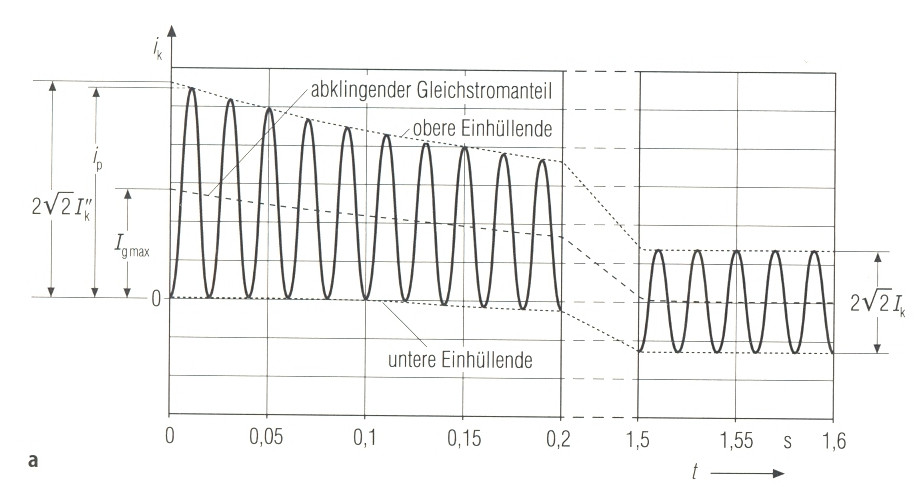
\includegraphics[scale=1.2]{img/kurzschlussstromverlauf-nah.jpg}
	\caption{Verlauf des generatornahen Kurzschlussstroms (Quelle: el. Kraftw. und Netze)}
	\label{kss-verlauf-nah}
	\end{figure}

Beim Eintritt des Kurzschlusses wird als erstes der subtransiente Anteil sichtbar. Er klingt bereits nach ein einigen Halbwellen exponentiell mit der Zeitkonstanten $T_d''$ ab und geht in den transienten Kurzschlussstrom über, welcher wesentlich langsamer abklingt. Überlagert wird der Kurzschlussstrom noch durch einen Gleichstromanteil. Dieser kommt dadurch zustande, dass durch die überwiegend induktive Kurzschlussreaktanz der Strom nicht \glqq springen\grqq{} kann. Aus diesem Grund wird ein Ausgleichsstrom $i_g$ erzwungen, welcher mit der Gleichstromzeitkonstanten $T_g$ abklingt. Die Höhe des Gleichstromgliedes ist abhängig vom Einschaltwinkel, also vom Einschaltzeitpunkt des Kurzschlusses, $\psi$ und ist bei $\psi = 0$ am größten.
%\\- Gleichstromglied \\

$i_k(t) = \sqrt{2} \cdot [(I_k'' - I_k') \cdot e^{-t/T_d''} + (I_k' - I_k) \cdot e^{-t/T_d'} + I_k] \cdot sin(\omega t + \psi - \varphi_k) + \sqrt{2} \cdot I_k'' \cdot e^{-t/T_g} \cdot sin( \varphi_k - \psi) $ \\


Vernachlässigt man die Resistanzen, ersetzt die Ströme und setzt $\psi = 0$, so gelangt man zu folgender Formel für den zeitlichen Verlauf: \\ \\
$i_k = \sqrt{2} \frac{U_n}{\sqrt{3}} [(\frac{1}{X_d''} - \frac{1}{X_d'}) e^{-t/T_d''} + (\frac{1}{X_d'} - \frac{1}{X_d}) e^{-t/T_d'} + \frac{1}{X_d}] \cdot cos(\omega t) + \sqrt{2} \frac{U_n}{\sqrt{3} X_d''} e^{-t/T_g}$ \\

Aus dieser Formel werden die drei überlagerten Anteile des Kurzschlussstromes deutlich. Auf die einzelnen Reaktanzen und Zeitkonstanten wird später genauer eingegangen. \\

Für den generatorfernen Kurzschluss gilt ähnliches. Da hier die Netzimpedanz allerdings einen wesentlich höheren Einfluss hat als beim generatorfernen Kurzschluss, kann noch weiter vereinfacht werden. Es wird $I_k'' = I_k' = I_k$ angenommen. Daraus ergibt sich nun folgende Formel: \\

$i_k(t) = \sqrt{2} \cdot I_k'' \cdot sin(\omega t + \psi - \varphi) + \sqrt{2} \cdot I_k'' \cdot e^{-t/T_g} \cdot sin(\varphi - \psi) $ \\

An dem Verlauf, der in Abbildung \ref{kss-verlauf-fern} dargestellt ist, erkennt man, dass der Kurzschlussstrom, insbesondere der Gleichanteil, wesentlich schneller abklingt als der generatornahe Kurzschluss. Die Zeitkonstanten $T_d''$ und $T_d'$ entfallen, es bleibt nur die Gleichstromzeitkonstante $T_g$.

	\begin{figure}[H]
	\centering
	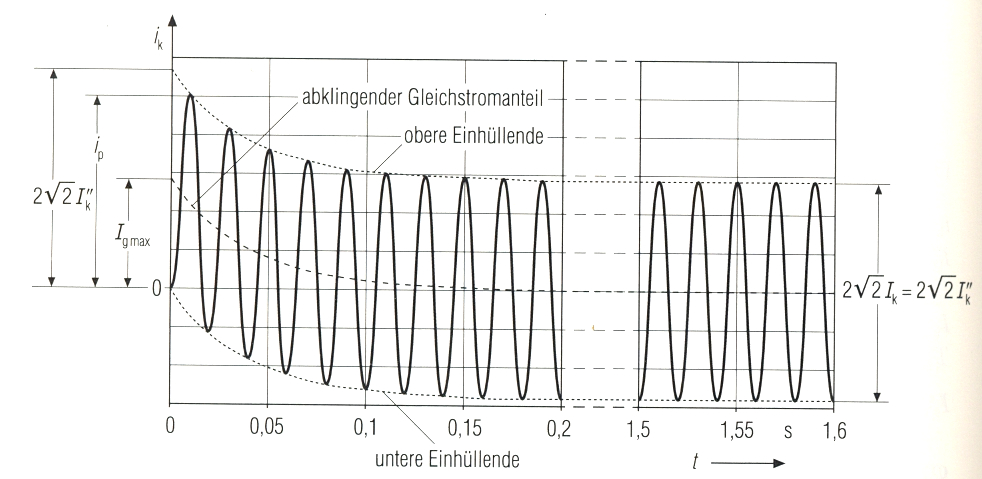
\includegraphics[scale=1]{img/kurzschlussstromverlauf-fern.jpg}
	\caption{Verlauf des generatorfernen Kurzschlussstroms (Quelle: el. Kraftw. und Netze)}
	\label{kss-verlauf-fern}
	\end{figure}
	
\subsection{Einpoliger Kurzschluss}
Einpolige Fehler mit Erdberührung sind die am häufigsten auftretenden Fehler in elektrischen Netzen (Quelle?). Sie entstehen beispielsweise durch herabfallende Äste oder durchhängende Vogelnester. Üblicherweise werden Netze bis 110kV kompensiert betrieben. Dabei wird der kapazitive Anteil des Stromes an der Fehlerstelle durch eine Petersenspule kompensiert, die zwischen dem Sternpunkt des Transformators und dem Erdreich angeschlossen wird. Kleinere Mittelspannungsnetze, beispielsweise in Industrieanlagen, werden auch mit isoliertem Sternpunkt betrieben. Netze mit höheren Spannungen werden starr geerdet. Man nennt dies \glqq Niederohmige Sternpunkterdung\grqq{} (NOSPE). Der Erdschlussstrom wird dann zu einem Erdkurzschlussstrom. Grundsätzlich wird unter folgenden Sternpunktbehandlungen unterschieden:

\begin{itemize}
\item Niederohmige Sternpunkterdung (NOSPE): Abbildung \ref{sternpunktbehandlung}a
\item Resonanzsternpunkterdung (RESPE): Abbildung \ref{sternpunktbehandlung}c
\item Isolierter Sternpunkt: Abbildung \ref{sternpunktbehandlung}b
\item Strombegrenzende Erdung: Abbildung \ref{sternpunktbehandlung}d
\end{itemize}
% Dadurch, dass der Fehlerstrom nicht kompensiert wird, löst der Schutz aus und der fehlerbehaftete Netzabschnitt wird sofort abgeschaltet.
%\\ Verlauf einpoliger Fehler?

	\begin{figure}[H]
	\centering
	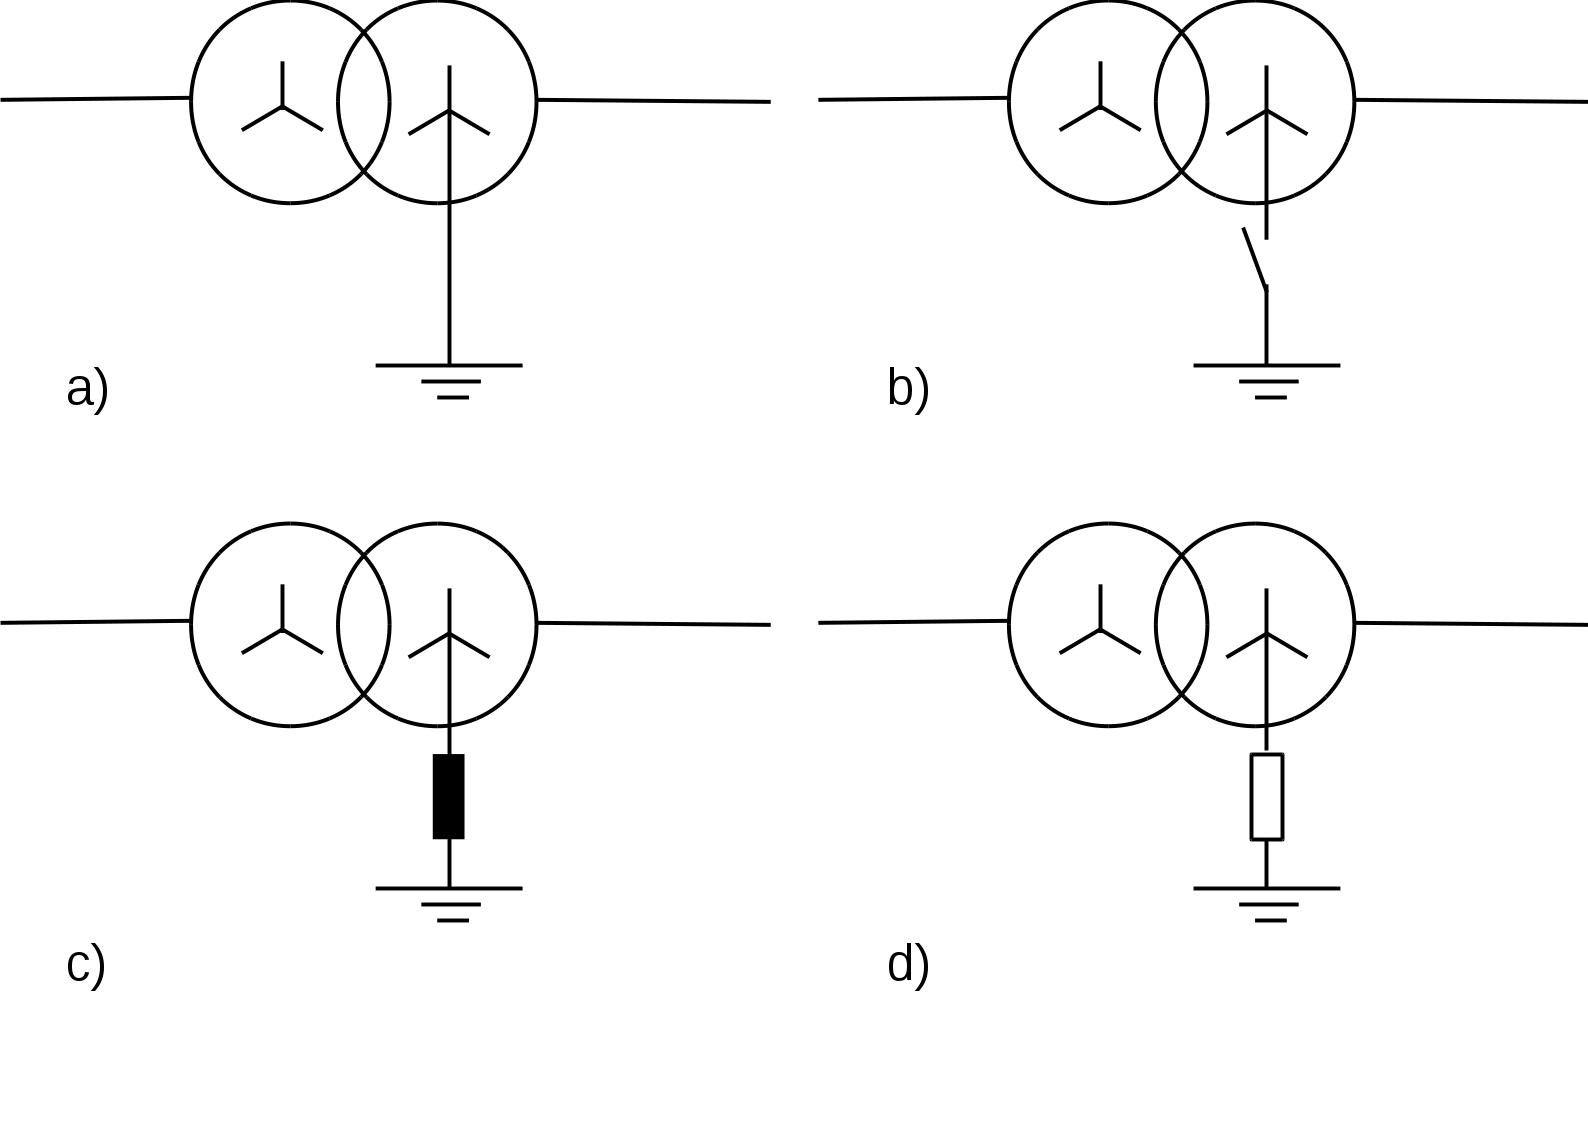
\includegraphics[scale=0.3]{img/sternpunktbehandlung.png}
	\caption{Sternpunktbehandlungen}
	\label{sternpunktbehandlung}
	\end{figure}

\subsubsection{Darstellung in symmetrischen Komponenten}
Da einpolige Fehler unsymmetrisch sind, müssen zur Berechnung symmetrische Komponenten hergezogen werden. In symmetrischen Komponenten sind einpolige Fehler eine Reihenschaltung aus Mit-, Gegen- und Nullsystem: \\

	\begin{figure}[H]
	\centering
	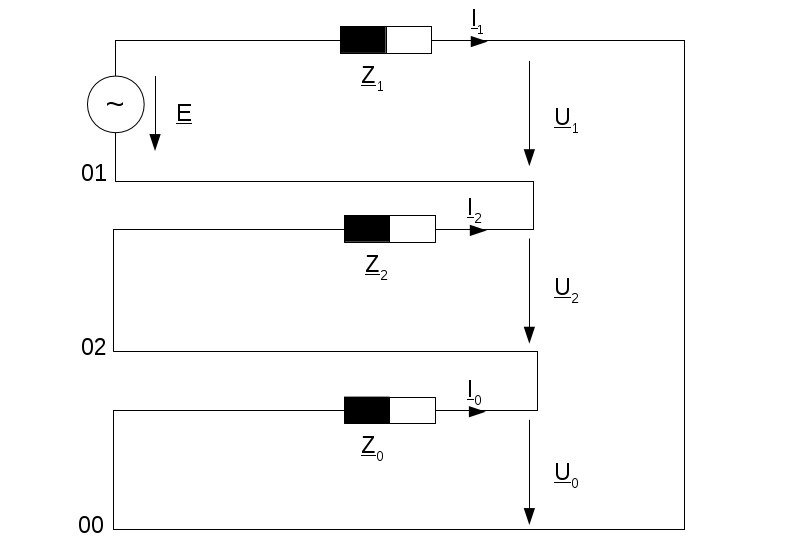
\includegraphics[scale=0.6]{img/einpol-fehler.png}
	\caption{Einpoliger Fehler in symmetrischen Komponenten}
	\label{einpol-fehler}
	\end{figure}
	
\subsubsection{Spannungserhöhung und Erdfehlerfaktor}
Zur Charakterisierung der Sternpunktbehandlung von elektrischen Netzen wird der Erdfehlerfaktor verwendet. Der Erdfehlerfaktor $\delta$ gibt dabei an, wie wirksam die Erdung ist. Eine Folge von einpoligen Fehlern ist die Erhöhung der Leiter-Erdspannung in den nicht fehlerbehafteten Leitern. Der Erdfehlerfaktor beschreibt dabei das Verhältnis zwischen der maximal auftretenden Leiter-Erdspannung $U_{LEmax}$ und der vor Fehlereintritt vorherrschenden Betriebsfrequenten Spannung $U^b$ geteilt durch $\sqrt{3}$. Ein Netz gilt dann als \glqq starr geerdet\grqq, wenn der Erdfehlerfaktor unter 1,4 bleibt. Gleichzeitig muss das Verhältnis von $X_0$ zu $X_1$ zwischen zwei und vier liegen (Sterpunktbehandlung S. 39). Bei der strombegrenzenden Sternpunkterdung ist die Nullimpedanz wesentlich größer, der Erdfehlerfaktor liegt zwischen 1,4 und $\sqrt{3}$.
% Das heißt, dass die Spannungsanhebung der fehlerfreien Leiter auf maximal das 1,4fache der vor Fehlereintritt auftretenden Spannung ansteigen darf. Dies wird vor allem bei Höchstspannungsnetzen angestrebt. Daraus lässt sich folgern, dass der Fehlerstrom umso höher ist, desto kleiner der Erdungswiderstand ist. Erhöht sich nun der Widerstand des Nullsystems, so lässt sich der Fehlerstrom verkleinern.

\subsection{Weitere Fehlerarten}
Neben dem dreipoligen und einpoligen Kurzschluss gibt es, wie bereits erwähnt, weitere Kurzschlussarten. Diese Fehler sind sogenannte \glqq Querfehler\grqq{}. Analog dazu werden Fehler, die durch Unterbrechung eines oder mehrerer Leiter entstehen, als \glqq Längsfehler\grqq{} bezeichnet. (Quelle?)

\subsection{Größen der Synchronmaschine}
Wie bereits dargestellt, ist die Kurzschlussimpedanz nicht konstant. Die Ursache dafür ist vor allem das Verhalten der Synchronmaschine. Da in konventionellen Kraftwerken ausschließlich Synchrongeneratoren zum Einsatz kommen, bestimmen diese maßgeblich den Verlauf des Kurzschlussstromes. Daher wird im folgenden Abschnitt näher auf die Synchronmaschine und ihre Größen eingegangen.

\subsubsection{Aufbau der Synchronmaschine}
Eine Synchronmaschine besteht, wie eine Asynchronmaschine, aus einem Ständer und einem Läufer. Der Aufbau des Ständers ist analog zur Asynchronmaschine. Bei einer Polpaarzahl von Eins sind in einem räumlichen Abstand von 120\degree{} um den Läufer drei Wicklungen angeordnet. Bei höheren Polpaarzahlen entsprechend sechs, neun, usw. Beim Aufbau des Läufers wird zwischen Schenkelpol- und Vollpolläufern unterschieden. Kleine und langsam laufende Generatoren (Laufwasserkraftwerke) bis ca. 300MVA besitzen meist einen Schenkelpolläufer. In großen schnell drehenden Kraftwerksgeneratoren sind Vollpolläufer verbaut, da Schenkelpolläufer nicht die enormen Fliehkräfte aushalten können. 
\\ (el. netze u. kraftwerke: S. 126 ff)

\subsubsection{d-q-Achse}
Die Reaktanz einer Synchronmaschine setzt sich aus einem Anteil der Längsachse (d-Achse) und einem Anteil der Querachse (q-Achse) zusammen. Bei der Schenkelpolmaschine ist die magnetische Leitfähigkeit der d-Achse größer als die der q-Achse, was zur Folge hat, dass Xd größer ist als Xq. Die ideale Vollpolmaschine ist mathematisch gesehen ein Sonderfall der Schenkelpolmaschine, bei der Xd = Xq ist. Für eine einfache Kurzschlussstromberechnung sind die Reaktanzen der d-Achse ausreichend. Will man jedoch dynamische Vorgänge simulieren, so werden die Reaktanzen der q-Achse ebenfalls benötigt. \\

	\begin{figure}[H]
	\centering
	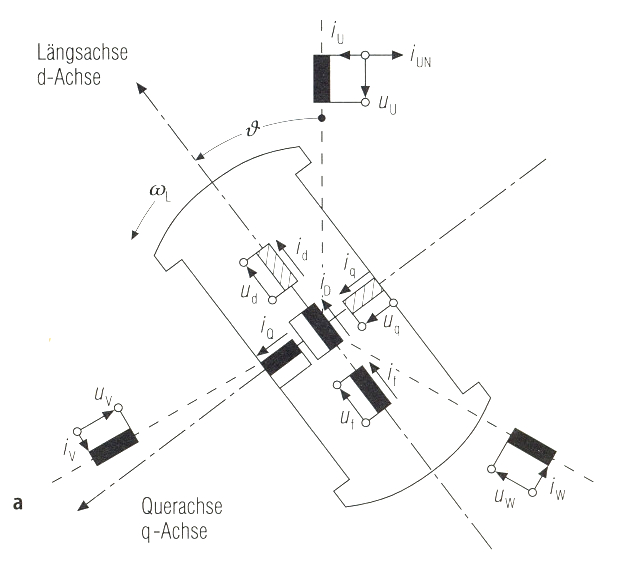
\includegraphics[scale=0.85]{img/schenkelpol.jpg}
	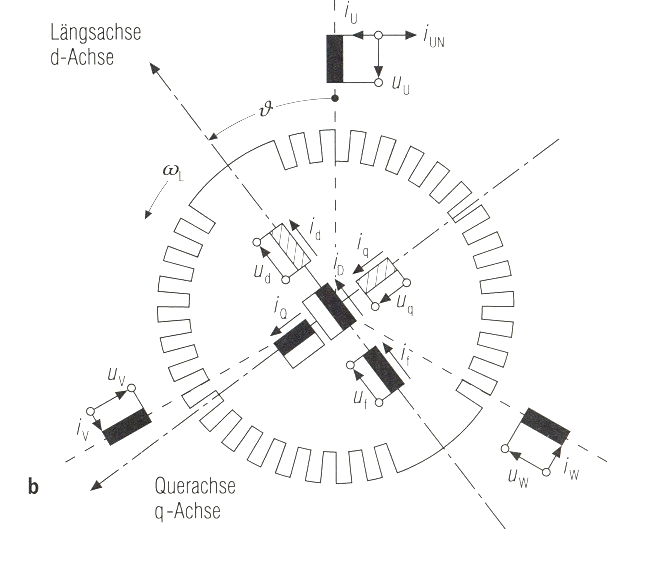
\includegraphics[scale=0.85]{img/vollpol.jpg}
	\caption{Querschnitt Schenkelpol- und Vollpolläufer (Quelle: el. Kraftw. und Netze)}
	\end{figure}

%	\begin{figure}[H]
%	\centering

%	\caption{test}
%	\end{figure}
%Ersetzt man nach der Zweiachsentheorie die drei Ständerwicklungen der Synchronmaschine durch zwei Ersatzwicklungen, so sind diese 90\degree elektrisch zueinander verschoben. Diese Komponenten auch als d-Achse (Längsachse) und q-Achse (Querachse) bezeichnet. Betrachtet man unsymmetrische Vorgänge, kommt noch eine 0-Komponente hinzu. Die Umrechnung der Drehstromkomponenten in dq0-Komponenten geschieht mit der Park-Transformation. Warum nur xd und kein xq bei KS-Berechnung?


\subsubsection{Subtransiente Reaktanz}
Um ersten Moment eines Kurzschlusses ist die subtransiente Reaktanz $X_d''$ wirksam. Mit ihr wird der Anfangskurzschlusswechselstrom berechnet. Ihr zugeordnet ist die subtransiente Zeitkonstante $T_d''$, welche das abklingen des Anfangskurzschlusswechselstromes beschreibt. Der Abklingvorgang wird mit einer e-Funktion beschrieben. Der gesamte subtransiente Vorgang dauert nur einige Halbwellen, danach geht der Kurzschluss in den transienten Vorgang über. Die Subtransientzeitkonstante $T_d''$ lässt sich wie folgt ermitteln: \\

$T_d'' = \frac{X_d'' + X_V}{X_d' + X_V} \cdot T_{d0}''$ \\

Dabei ist $T_{d0}''$ die Subtransient-Leerlaufzeitkonstante und liegt bei etwa 50ms.



\subsubsection{Synchrone Reaktanz}
Die synchronen Reaktanz $X_d$ gibt die wirksame Reaktanz während des stationären Betriebs an. Sie ist auch nach dem Abschluss aller Ausgleichvorgänge wirksam, daher kann mit ihr der Dauerkurzschlussstrom ermittelt werden. Die Reaktanz der q-Achse wird entsprechend mit $X_q$ bezeichnet.

\subsubsection{Transiente Reaktanz}
Während des transienten Vorgangs, der wesentlich langsamer Abklingt als der subtransiente Vorgang, ist die transiente Reaktanz $X_d'$ wirksam.

\subsubsection{Gegensystem}
Die Gegenreaktanz der Synchronmaschine kann ungefähr aus dem Mittelwert von $x_d''$ und $x_q''$ bestimmt werden: \\ \\
$x_i = \frac{x_d'' + x_q''}{2}$

\subsubsection{Nullsystem}
Da Synchronmaschinen symmetrisch aufgebaut sind, ist das Nullsystem theoretisch nicht wirksam. In der Praxis tritt die Nullreaktanz allerdings mit einer Größe von \\
$x_0 = \frac{1}{3} … \frac{1}{6} \cdot x_d'$ auf. Diese ist nur wirksam, wenn der Sternpunkt des Generators geerdet ist.

\subsubsection{Polradwinkel}
Der Polradwinkel, auch Lastwinkel genannt, gibt die Phasenverschiebung zwischen Polradspannung $U_p$ und Netzspannung an. Mechanisch gesehen ist er die mechanische Verschiebung des Polrads zwischen Leerlauf und Last. Jeder Leistung ist dabei ein Lastwinkel zugeordnet. Befindet sich die Maschine im Generatorbetrieb, eilt das Polrad vor und \glqq zieht\grqq{} das Netz mit. Arbeit die Maschine als Motor, eilt das Polrad nach und wird vom Netz \glqq mitgezogen\grqq.


\subsection{Stabilität}
Das Kriterium der Stabilität eines elektrischen Netzes unterscheidet zwischen der statischen Stabilität und der transienten Stabilität. Die statische Stabilität beschreibt.

Der Polradwinkel eines Generators hat einen entscheidenden Einfluss auf die Stabilität.

Die transiente Stabilität beschreibt das Verhalten des Netzes im Moment eines Fehlereintritts und danach.

Treten in einem Netz Fehler auf, so ändern sich die Lastflussverhältnisse und somit auch die abgegebene Leistung der Generatoren. Ein Spannungseinbruch, beispielsweise als Folge eines Kurzschlusses, führt zu einem schlagartigen Abfall der Last an einem Generator. Da die elektrische Energie nun nicht mehr ins Netz abgeführt werden kann, an der Welle aber immer noch mechanische Energie zugeführt wird, wird diese mechanische Energie in Rotationsenergie umgewandelt (???). Der Generator beschleunigt. Durch die Beschleunigung des Generators vergrößert sich der Polradwinkel. Wird dieser zu groß und überschreitet die Stabilitätsgrenze (wo liegt die?), gerät der Generator \glqq außer Tritt\grqq, wodurch es zu Schäden kommen kann. Diese liegt bei einem Polradwinkel von $\upsilon = 90\degree$ und markiert das Kippmoment $M_k$ der Maschine (S 187 el. Energieversorgung). Umso länger der Fehler andauert und umso näher der Fehler in der Nähe eines Genertors liegt, desto weniger Energie können die Generatoren ins Netz abführen. Die Wahrscheinlichkeit, dass ein Generator \glqq durchtritt\grqq, steigt also mit der Kurzschlussdauer an. Generatornahe Fehler müssen daher besonders schnell abgeschaltet werden. Durch ein schnelles erhöhen der Generatorspannung kann erreicht werden, dass im Fehlerfall mehr Wirkleistung abgeführt werden kann. Kleinere Spannungsänderungen im Netz führen, wie bereits beschrieben, zu Leistungsänderungen an den Generatoren. Diese führen in der Regel nicht zu Instabilitäten, allerdings pendelt nun das Polrad mit einer niedrigen Frequenz von bis zu 2 Hz. Diese Leistungspendelungen sind auch im Netz beobachtbar, vor allem zwischen schwach gekoppelten Netzen (Wide Area Monitoring System UCTE). Sichtbar gemacht werden diese mit Wide Area Monitoring Systems.

Die Stabilität eines Drehstromnetzes ist ein wesentliches Kriterium zur Versorgungssicherheit.

%- S. 902 \\
%- niederfrequente netzpendelungen \\
%- statisch \\
%- transient \\
%- Zeit zum durchgehen \\


\section{PSS Sincal}

\subsection{Lizenzen}
Die Fachhochschule Bielefeld besitzt unterschiedliche Lizenzen für die PSS Sincal Plattform. Mit allen Lizenzen können Kurzschlüsse, Lastflüsse und die Stabilität untersucht werden. Die EduTrans-Lizenz ist hier auf maximal 25 gleichzeitige Nutzer begrenzt. Mit dieser Lizenz können ferner Schutzfunktionalitäten und Oberschwingungen untersucht werden. Elektromagnetische Transienten und zeitliche Verläufe von Momentanwerten können allerdings nicht dargestellt werden. Die Lizenz EleStd ermöglicht dagegen auch die Untersuchung von elektromagnetischen Transienten und Eigenwerten. Hier fehlt allerdings Funktion der Schutzkoordination. EleStd ist auf sechs gleichzeitige Nutzer begrenzt. \\
Des weiteren verfügt die Fachhochschule über zwei EleKey2-Lizenzen, welche im Gegensatz zu den Netzwerklizenzen auf einen USB-Dongle setzt. Diese Lizenzen enthalten die selben Funktionen wie die EleStd-Lizenz

\subsection{Netz}
Das Netz, welches im Praktikum verwendet wird, ist im Anhang in Abbildung \ref{praktikum-netz} abgebildet. Es ist ein starr geerdetes 110kV-Freileitungsnetz, welches vermascht ist. Als Einspeisequellen dienen zwei räumlich unterschiedlich angeordnete Synchrongeneratoren mit Leistungen von 100MVA und 80MVA, sowie das überlagerte 380kV-Netz. Die Netzdaten wurden von den Praktikumsunterlagen \glqq ENE 3 Kurzschlussstromberechnung in elektrischen Netzen\grqq{} übernommen. Die Dynamikdaten der Generatoren wurden aus den Praktikumsunterlagen der Otto-von-Guericke-Universität Magdeburg übernommen.

\section{Simulation mit NETOMAC}
PSS NETOMAC ist eine leistungsfähige Software zur Untersuchung von dynamischen Vorgängen in elektrischen Netzen. Es wird von der Firma Siemens entwickelt und vertrieben.

\subsection{Export aus PSS Sincal}
Über die Exportfunktion von PSS Sincal lässt sich aus einem Sincal-Projekt ein Netomac-Projekt erstellen. Sie findet sich unter $Datei \rightarrow Exportieren \rightarrow PSS$ $NETOMAC...$ .  Nach dem erfolgreichen Export erhält man unter anderem  Dateien mit folgenden Dateiendungen:

\begin{itemize}
\item .nprj: Projektdatei
\item .ctl: Steuerungsdatei
\item .net: Hauptdatei mit Netzaufbau
\item .nzd: Datei mit Namen und Aliasnamen
\item .dis: Störungsdatendatei
\item .plo: Plotterdatendatei
\item .res: Ergebnisdatei
\end{itemize}


\subsection{.ctl-Datei}
In der .ctl-Datei werden allgemeine Einstellungen festgelegt, wie z.B. der Simulationszeitraum und der Zeitschritt. Des weiteren werden dort die Suchpfade festgelegt, in denen NETOMAC benötigte Dateien suchen soll.

\subsection{.net-Datei}
In der .net-Datei sind alle Betriebsmittel, Knoten und Zweige und die Netztopologie definiert. Jedes Betriebsmittel und jeder Knoten hat eine eindeutige Bezeichnung, aus der nicht direkt ersichtlich ist, um welche Art von Betriebsmittel es sich handelt. In jeder Definition eines Betriebsmittels sind der Anfangsknoten und der Endknoten definiert. Nachfolgend ist in Tabelle \ref{leitung-netomac-tb} die Definition einer Leitung dargestellt, an der die Funktionsweise von NETOMAC demonstriert wird.

\begin{table}[H]
\begin{tabular}{|l|l|l|l|l|l|l|l|l|l|l|l|}
\hline 
\multicolumn{12}{|l|}{\$ Line: L12 (X00028) from SS1 (X00005) to SS2 (X00006)} \\ 
\hline 
LX00005 & X00006  & X00028 & 1 & 30 & 0.116 & 0.424 & 9.17 & 0 & 110 & 0 &0 \\ 
\hline 
M & & X00028 & & 9999 & 9999 & & & & & & \\ 
\hline 
\end{tabular} 
\caption{Definition einer Leitung in PSS NETOMAC}
\label{leitung-netomac-tb}
\end{table}

Netomac arbeiten mit einem tabellenartigen Textformat, Spalten sind dabei durch Tabulatoren getrennt. Die Kennzeichnung von Zeilen geschieht durch Buchstaben, wobei jeder Buchstabe eine andere Funktion hat. Die Eigenschaften der Zeile wird anschließend in den Spalten festgelegt.

Alle Zeilen, die mit einem \$ beginnen, sind Kommentare. Beim Export von PSS Sincal in PSS Netomac versieht Sincal automatisch alle Betriebsmittel mit Kommentaren. Knoten- und Betriebsmittelkennzeichnungen beginnen mit X und haben eine eindeutige alphanumerische Bezeichnung. In diesem Beispiel hat die Leitung L12 die Bezeichnung X00028 und verbindet die Knoten X00006 und X00028 miteinander. Die Zeile mit der Bezeichnung L kennzeichnet eine Leitung, anschließend folgt ohne Leerzeichen die Bezeichnung des Anfangsknotens (X00005). In der nächsten Spalte folgt nach einem Tabulator die Bezeichnung des Endknotens (X00006), anschließend die Bezeichnung der Leitung selbst. Ab hier beginnen die eigentlichen Parameter der Leitung. Zunächst wird die Anzahl der parallelen Leitungen festgelegt, in diesem Fall 1. Die Länge ist mit 30km definiert. Anschließend werden die Resistanz R' mit 0,116 $\Omega /km$, die Reaktanz mit 0,424 $\Omega /km$ und die Kapazität $C_b'$ mit 9,17nF/km festgelegt. Da in der Versuchsbeschreibung kein Wert für $C_0'$ gegeben war, ist dieser Null. Die Nennspannung auf der Leitung beträgt 110kV. Für die Ableitwiderstände gilt dasselbe wie für $C_0'$, daher wurden $G_1'$ und $G_0'$ auch zu Null.\\
In der Zeile mit der Bezeichnung M wird die Kopplung zwischen dem Mit- und Nullsystem definiert. Spalte zwei und drei sind leer, in der vierten Spalte wird die Bezeichnung der Leitung angegeben, für die die Kopplung definiert werden soll, in diesem Fall X00028. Da auch hier keine Werte gegeben sind, setzt Sincal die beiden folgenden Spalten, welche für das Verhältnis $R_0'/R_b'$ und $X_0'/X_b'$ stehen, auf 9999. Das bedeutet, dass die beiden Werte für $X_0'$ und $R_0'$ praktisch nicht vorhanden sind. Nachfolgend ist in Abbildung \ref{leitung-netomac} die Leitung L12, wie in Tabelle \ref{leitung-netomac-tb} beschrieben, noch einmal im Texteditor von NETOMAC dargestellt.

	\begin{figure}[H]
	\centering
	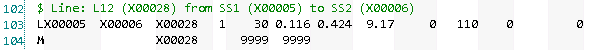
\includegraphics[scale=0.75]{img/netomac-l12.png}
	\caption{Definition der Leitung L12 in NETOMAC}
	\label{leitung-netomac}
	\end{figure}
	
Da in die Betriebsmittelbezeichnungen in der .net-Datei kryptisch und ohne Bezug sind, hat NETOMAC die Möglichkeit von Aliasnamen eingeführt. Diese sind in der Datei mit der Endung .nzd definiert. PSS Sincal legt automatisch Aliases mit den in Sincal angegebenen Namen an. \\
Generatoren werden nach dem selben Prinzip beschrieben. Zeile S kennzeichnet eine Synchronmaschine. Da dieses Betriebsmittel keinen Anfangs- und Endknoten hat, bleiben die nachfolgenden zwei Spalten leer. In der dritten Spalte folgt wie üblich die Bezeichnung des Betriebsmittels. Zeile T legt die Transformator-Parameter fest. Da der Generator und der Transformator separat betrachtet werden und nicht als Kraftwerksblock, ist das Übersetzungsverhältnis 1. Die Schaltgruppe des Synchrongenerators ist YY0, was bedeutes, dass die Ständerwicklungen im Stern verschaltet sind. Da das Übersetzungsverhältnis 1 ist, sind die nachfolgenden Angaben für $U_{r,UStrafo}$, $U_{nUStrafo}$ und $U_{nOSnetz}$ jeweils 10kV. Die Bemessungsspannung des Synchrongenerators beträgt allerdings 10,5kV. Die nachfolgende Zeile definiert die Nennwerte der Maschine. Auf die Scheinleistung in MVA folgt die Wirkleistung, die Nennspannung, der Leistungsfaktor, der Wirkungsgrad, die Nenndrehzahl und die Nennfrequenz. In Zeile zwei bis sechs sind die Parameter des Ersatzschaltbildes der Maschine definiert. Die Z-Zeile beinhaltet weitere Parameter, die zur Kurzschlussberechnung nach IEC und ANSI benötigt werden.

	\begin{figure}[H]
	\centering
	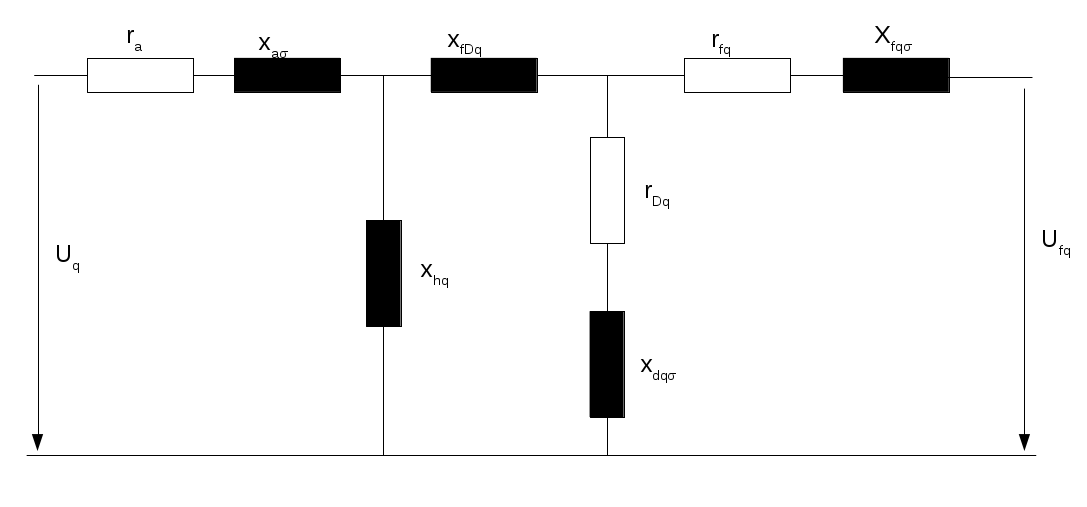
\includegraphics[scale=0.5]{img/esb-synchron.png}
	\caption{Ersatzschaltbild Synchrongenerator}
	\label{leitung-netomac}
	\end{figure}

	\begin{figure}[H]
	\centering
	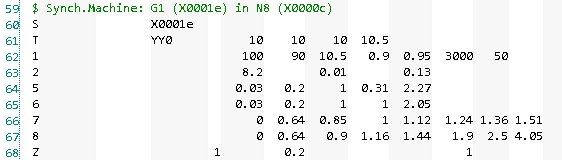
\includegraphics[scale=0.75]{img/netomac-g1.png}
	\caption{Definition des Synchrongenerator G1 in NETOMAC}
	\label{leitung-netomac}
	\end{figure}

\subsection{.dis-Datei}
In der .dis-Datei (\glqq disturbance\grqq) werden die Störkriterien und Netzänderungen festgelegt. Einzelne Ereignisse können dabei sequenziell oder parallel ablaufen. Jedes Ereignis kann aus mehreren Störkriterien bestehen und beginnt mit einer Einleitungszeile. Die Einleitungszeile dient dazu, NETOMAC kenntlich zu machen, das ein neues Ereignis stattfindet. In ihr wird die Zeit angegeben, nach der das nächste Ereignis ausgeführt werden soll. Nach der Einleitungszeile folgen Fehlerzeilen. Jede Fehlerzeile definiert dabei den Fehlerort, die Art des Fehlers, die Fehlerimpedanz und eventuell eine Fehlerimpedanz gegenüber Erde. Das Ereignisende erfolgt eine \glqq ENDE\grqq -Zeile. Nun kann das nächste Ereignis definiert werden. Soll das Netz in den Ausgangszustand zurückversetzt werden, geschieht dies mit einer \glqq OLD\grqq -Zeile, gefolgt von einer \glqq ENDE\grqq -Zeile. 

\subsection{.plo-Datei}
In der Plotterdatei wird definiert, welche Signale aufgenommen werden sollen. Dies kann auch komplett über ein grafisches Menü geschehen, was wesentlich komfortabler ist als die reine Texteingabe.

%\subsection{.res-Datei}

\subsection{Dateistruktur}
\subsection{Eingabedaten}

\subsection{Berechnungsmethoden}
PSS NETOMAC bietet drei unterschiedliche Berechnungsmethoden an

\subsubsection{Lastfluss}


\subsubsection{Kurzschluss}
Kurzschlüsse können in NETOMAC wahlweise nach ANSI oder IEC bzw. VDE0102 berechnet werden.


\subsubsection{Dynamik}
Die Dynamikberechnungen bilden die mit Abstand größte Funktionsvielfalt in NETOMAC. Mit ihr lassen sich zum einen die Stabilität eines Netzes und zum anderen elektromagnetische Transienten berechnen und grafisch darstellen.

\subsection{Vierpoldarstellung von Leitungen}
Bei einfachen Kurzschlussstromberechnungen wird bei elektrischen Leitungen der Querzweig vernachlässigt und nur der Längszweig mit Induktivitäten und Resistanzen betrachtet. Dies führt bei der Auslegung von Betriebsmitteln zu hinreichend genauen Ergebnissen. Werden nun aber dynamische Vorgänge betrachtet, lassen sich die Querzweige nicht mehr vernachlässigen und müssen in die Betrachtungen mit einfließen.

\subsubsection{Vollständiges Ersatzschaltbild}


\subsubsection{$\pi$-Ersatzschaltbild}
Bis zu einer Leitungslänge von ca. 150km (el. Energieversorgung S. 216) liefert das $\pi$-Ersatzschaltbild ein realistisches Übertragungsverhalten. Bei längeren Leitungen müssen mehrere Pi-Glieder hintereinander geschaltet werden. Der Vorteil am $\pi$-Ersatzschaltbild ist, dass es keine inneren Knoten besitzt und dadurch Rechnungen stark vereinfacht (Quelle?).

	\begin{figure}[H]
	\centering
	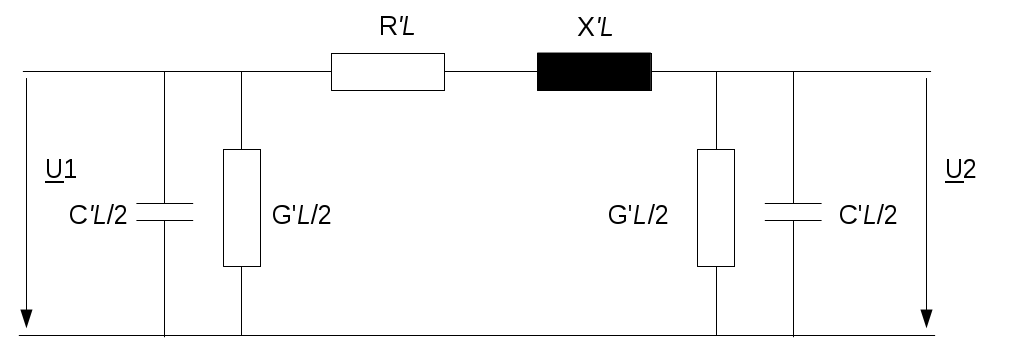
\includegraphics[scale=0.5]{img/pi-esb.png}
	\caption{$\pi$-Ersatzschaltbild Leitung}
	\label{pi-esb}
	\end{figure}

\subsubsection{T-Ersatzschaltbild}
Das $\pi$-Ersatzschaltbild hat bei dynamischen Betrachtungen den Nachteil, dass sich an seinen Enden Kapazitäten befinden, die im Kurzschlussfall zusammen mit der Induktivität einen nur schwach gedämpften Schwingkreis bilden. Dies führt bei der grafischen Darstellung zu \glqq Spikes\grqq{}, die in der Realität nicht vorkommen. Tritt dieser Fall auf, so liefert das T-Ersatzschaltbild realistischere Ergebnisse (Netomac-Hilfe). Sichtbar wird dies bei einem Vergleich der Abbildungen \ref{u-pi} und \ref{u-t}. Diese zeigen den Spannungsverlauf bei einem dreipoligen Kurzschluss auf der Leitung L67 an der Sammelschiene SS6. Wie zu erkennen, sind die \glqq Spikes\grqq{} beim T-Ersatzschaltbild wesentlich kleiner.

	\begin{figure}[H]
	\centering
	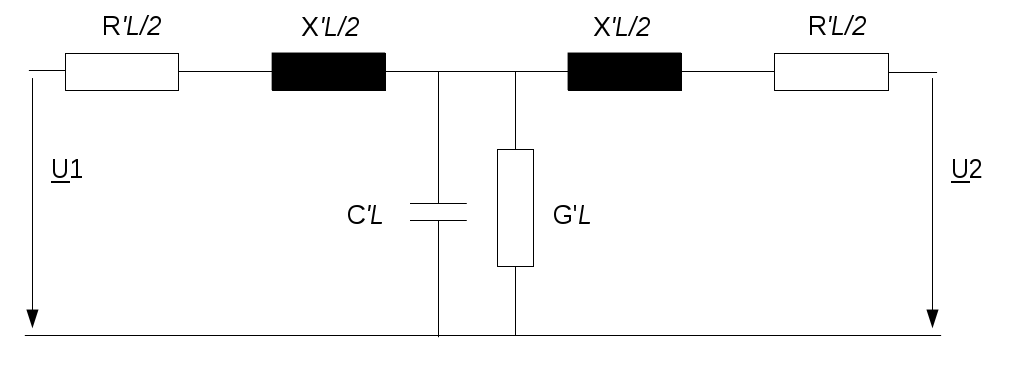
\includegraphics[scale=0.5]{img/t-esb.png}
	\caption{T-Ersatzschaltbild Leitung}
	\label{t-esb}
	\end{figure}
	
	\begin{figure}[H]
	\centering
	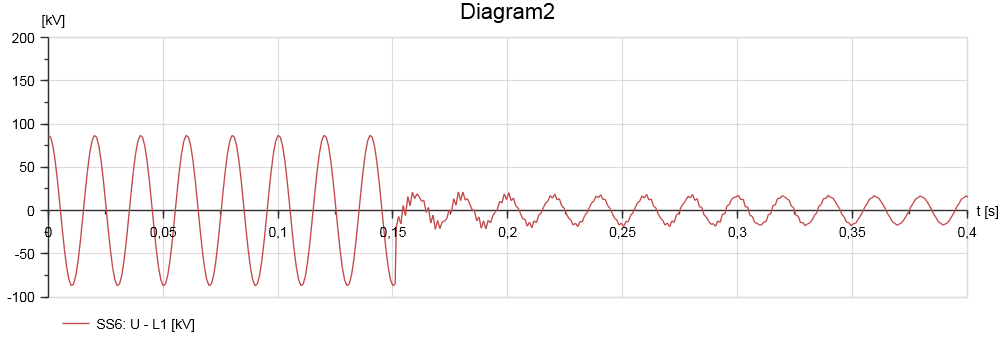
\includegraphics[scale=0.45]{img/u-pi.png}
	\caption{Spannung an SS6 mit PI-ESB}
	\label{u-pi}
	\end{figure}
	
	\begin{figure}[H]
	\centering
	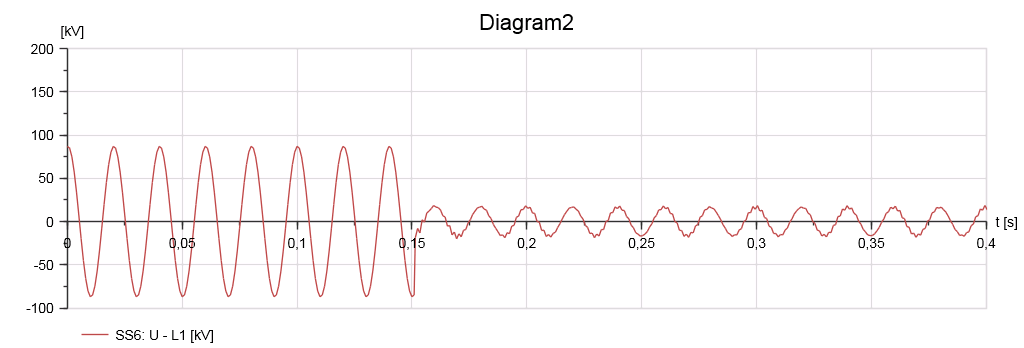
\includegraphics[scale=0.45]{img/u-t.png}
	\caption{Spannung an SS6 mit T-ESB}
	\label{u-t}
	\end{figure}

\subsection{Festlegen der Störkriterien}
\subsection{Grafische Auswertung}

\section{Prüfgerät Kocos Artes}
\subsection{COMTRADE}
Das COMTRADE-Datenformat ist ein Standard zum Aufzeichnen von transienten Signalen, beispielsweise von Störungen in elektrischen Netzen. Diese können dann mit gängigen Programmen grafisch dargestellt und weiterverarbeitet werden. Eine Anwendungsmöglichkeit ist die Fehleranalyse von Störungen, die durch ein Versagen des Schutzgerätes verursacht werden. Dazu wird mit einem Prüfgerät, z.B. mit einem Kocos Artes oder einer Omicron CMC, die COMTRADE-Datei der Störung \glqq abgespielt\grqq{} und die Spannungen und Ströme auf das vermeintlich defekte Schutzgerät gegeben. So lassen sich die Auslösekennlinien im Labor mit echten Daten überprüfen.

\section{Überarbeitung Laborunterlagen}
\section{Zusammenfassung}

\newpage
\pagenumbering{Roman}
\setcounter{page}{1}
\section{Literaturverzeichnis}
\bibliography{bibtest1}
\bibliographystyle{unsrtdin}

\section{Anhang}
\subsection{Netz Laborversuch}
\begin{table}[H]
\begin{tabular}{|c|c|}
\hline 
\textbf{Bezeichnung} & \textbf{Netz 1} \\ 
\hline 
Kurzschlussleistung $S_k''$ & 1000MVA \\ 
\hline 
Kurzschlussleistung $S_k''$ Maximum & 1000 \\ 
\hline 
Kurzschlussleistung $S_k''$ Minimum & 1000 \\ 
\hline 
Verhältnis R/X & 0.1 p.u. \\ 
\hline
\end{tabular} 
\caption{Nenndaten des starren Netzes}
\end{table}

\begin{table}[H]
\begin{tabular}{|c|c|c|}
\hline 
\textbf{Bezeichnung} & \textbf{Transformator 1} & \textbf{Transformator 2} \\ 
\hline 
Nennspannung Seite 1 $U_{n1}$ & 110kV & 110kV \\ 
\hline 
Nennspannung Seite 2 $U_{n2}$ & 10kV & 10kV \\ 
\hline 
Nennscheinleistung $S_n$ & 100MVA & 80MVA \\ 
\hline 
Dauerleistung $S_{max}$ & 100MVA & 80MVA \\ 
\hline 
Kurzschlussspannung $u_k$ & 12\% & 12\% \\ 
\hline 
Ohmsche Kurzschlussspannung $u_r$ & 0,38\% & 0,38\% \\ 
\hline 
Schaltgruppe & Yy0 & Yy0 \\ 
\hline 
\end{tabular}
\caption{Nenndaten Transformatoren}
\end{table}

\begin{table}[H]
\begin{tabular}{ll}

\begin{tabular}{|c|c|}
\hline 
\textbf{Bezeichnung} & \textbf{Kenndaten} \\ 
\hline 
Leitungstyp & Freileitung \\ 
\hline 
Widerstand r & 0,118 Ohm/km \\ 
\hline 
Reaktanz x & 0,421 Ohm/km \\ 
\hline 
Kapazität c & 9,17nF/km \\ 
\hline 
Nennspannung & 110kV \\ 
\hline 
Therm. Grenzstrom & 645A \\ 
\hline 
\end{tabular}

&

\begin{tabular}{|c|c|}
\hline 
\textbf{Leitung} & \textbf{Länge} \\ 
\hline 
L12 & 30km \\ 
\hline 
L16 & 50km \\ 
\hline 
L23 & 45km \\ 
\hline 
L25 & 30km \\ 
\hline 
L34 & 25km \\ 
\hline 
L45 & 20km \\ 
\hline 
L64 & 35km \\ 
\hline 
L67 & 20km \\ 
\hline 
\end{tabular}

\end{tabular}

\caption{Freileitungen}
\end{table}

\begin{table}[H]
\begin{tabular}{|c|c|c|}
\hline 
\textbf{Last} & \textbf{Scheinleistung} & \textbf{Leistungsfaktor} \\ 
\hline 
Last 1 & 40MVA & 0,95 \\ 
\hline 
Last 2 & 30MVA & 0,8 \\ 
\hline 
Last 3 & 60MVA & 0,9 \\ 
\hline 
Last 5 & 40MVA & 0,9 \\ 
\hline 
Last 7 & 60MVA & 0,9 \\ 
\hline 
\end{tabular}
\caption{Lasten}
\end{table}

\begin{table}[H]

\begin{tabular}{|l|c|c|}
\hline 
\textbf{Bezeichnung} & \textbf{Generator 1} & \textbf{Generator 2} \\ 
\hline 
Maschinentyp & Turbogenerator & Turbogenerator \\ 
\hline 
Bemessungsscheinleistung & 100MVA & 80MVA \\ 
\hline 
Bemessungsspannung & 10kV & 10kV \\ 
\hline 
Verhältnis R/X & 0,1 p.u. & 0,1 p.u. \\ 
\hline 
Anlaufzeitkonstante $T_A$ & 8,2s & 8,2s \\
\hline
Gleichstromzeitkonstante $T_G$ & 0,36s & 0,36s \\
\hline
Ankerwiderstand $R_a$ & 0,01 p.u. & 0,01 p.u. \\
\hline
Ankerstreureaktanz $X_{1\sigma}$ & 0,13 p.u. & 0,13 p.u. \\
\hline
\multicolumn{3}{|l|}{Kurzschlusszeitkonstanten} \\
\hline
• subtransient d-Achse $T_d''$ & 0,03s & 0,03s \\
\hline
• subtransient q-Achse $T_q''$ & 0,03s & 0,03s \\
\hline
• transient d-Achse $T_d'$ & 1,0s & 1,0s \\
\hline
• subtransient q-Achse $T_q'$ & 1,0s & 1,0s \\
\hline
\multicolumn{3}{|l|}{Reaktanzen} \\
\hline
• subtransient d-Achse $X_{d}''$ & 20\% & 20\% \\ 
\hline
• subtransient q-Achse $X_q''$ & 20\% & 20\% \\
\hline
• transient d-Achse $X_{d}''$ & 30,1\% & 30,1\% \\ 
\hline
• transient q-Achse $X_q''$ & 100\% & 100\% \\
\hline
• stationär d-Achse $X_d$ & 227\% & 227\% \\
\hline
• stationär q-Achse $X_q$ & 205\% & 205\% \\
\hline
Bemessungsleistungsfaktor & 0,9 & 0,9 \\ 
\hline 
Wirkleistung P & 90MW & 72MW \\ 
\hline 
Generatorspannung & 10kV & 10kV \\ 
\hline
\end{tabular}

\caption{Generatoren}
\end{table}


	\begin{figure}[H]
	\centering
	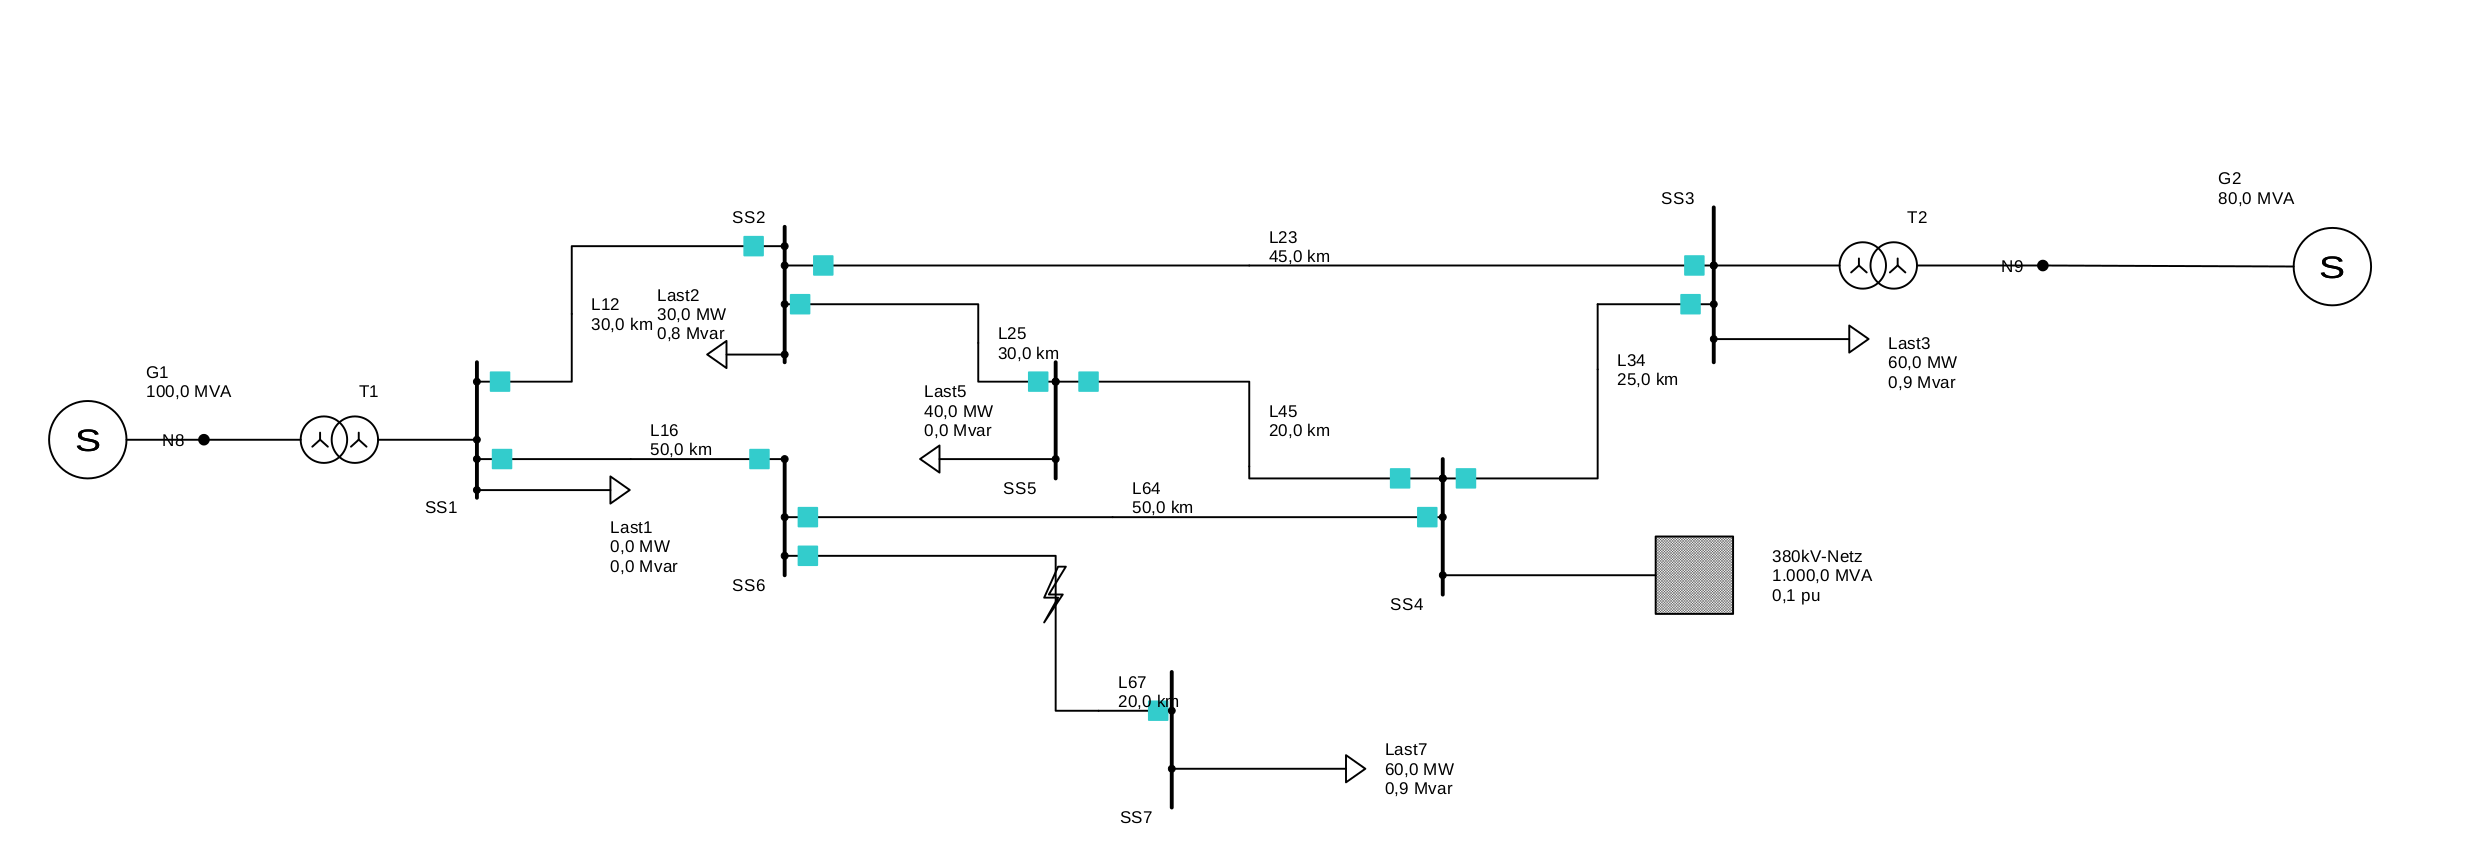
\includegraphics[scale=0.35, angle=90]{img/praktikum-netz}
	\caption{Netzaufbau Laborversuch}
	\label{praktikum-netz}
	\end{figure}
	
\subsubsection*{Dateien auf DVD}
\begin{itemize}
\item Bachelorarbeit.pdf
\item comtrade-adjust.vbscript
\item Sincal-Projekt Kurzschlussversuch
\item Überarbeiteter Laborversuch
\end{itemize}

\end{onehalfspace}

\end{document}

